% ******************************* Thesis Appendix B ********************************

\chapter{Supporting information: Chapter 5}

\graphicspath{{Appendix4/Figures/}}

\section{Supplementary figures and tables}
\newpage
\begin{figure}[H]
\flushleft{\textbf{Figure S5.1.} Positive pairwise species correlations to the environment derived from single-predictor LVMs for the full dataset. Connecting lines between species nodes denote positive mean posterior correlations with credible intervals excluding zero. Line colour and thickness indicates the strength of the positive correlation where darker and thicker lines are closer to 1. Species node labels combine the first letters of the genus and specific epiphet.}
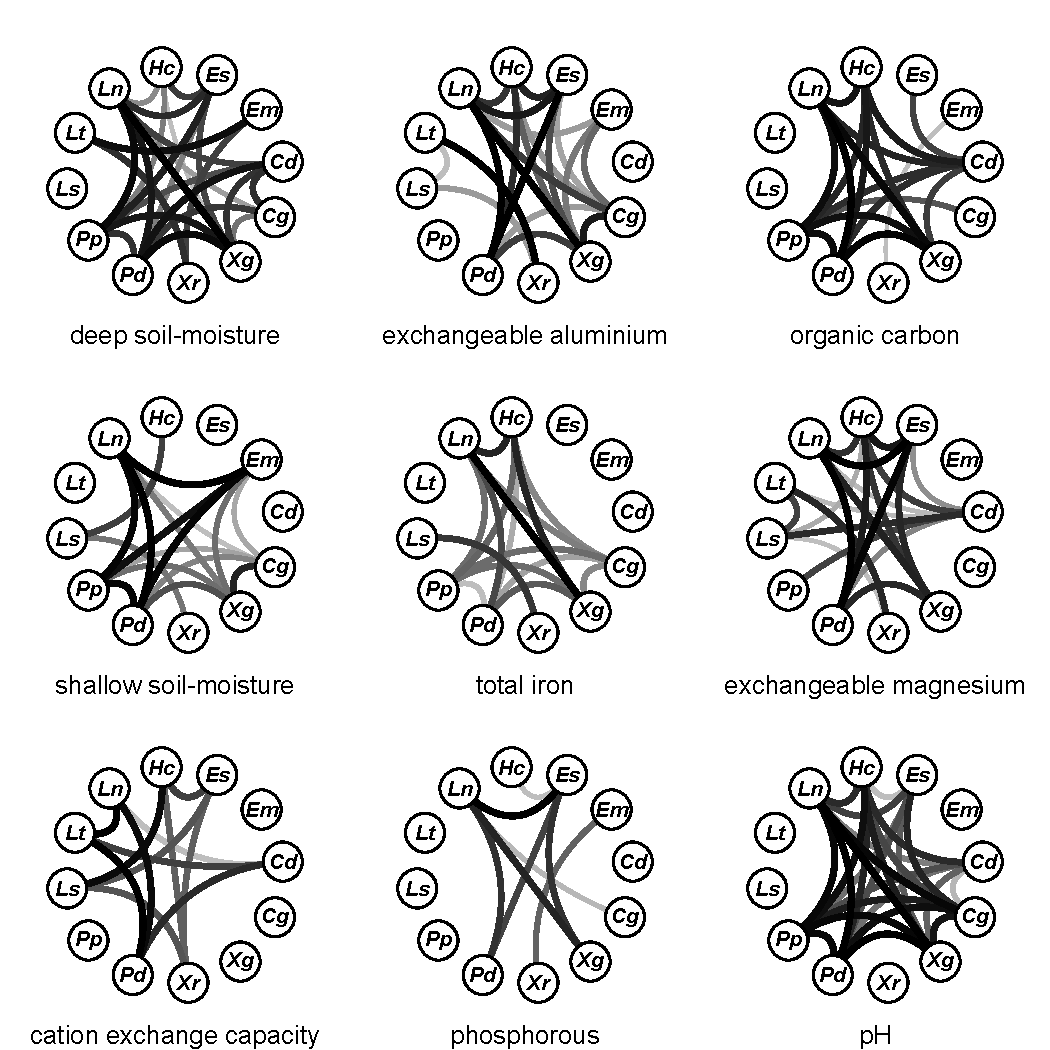
\includegraphics[width=1.0\linewidth]{networkplots-positive-unshrink}\\
\end{figure}

\begin{figure}[H]
\flushleft{\textbf{Figure S5.2.} Abundance of each species (excl. \textit{Empodisma minus}) through time. Trend lines obtained with thin-plate splines in a GAMM framework (see main text for model fitting). Shaded region represents 95\% confidence intervals.}
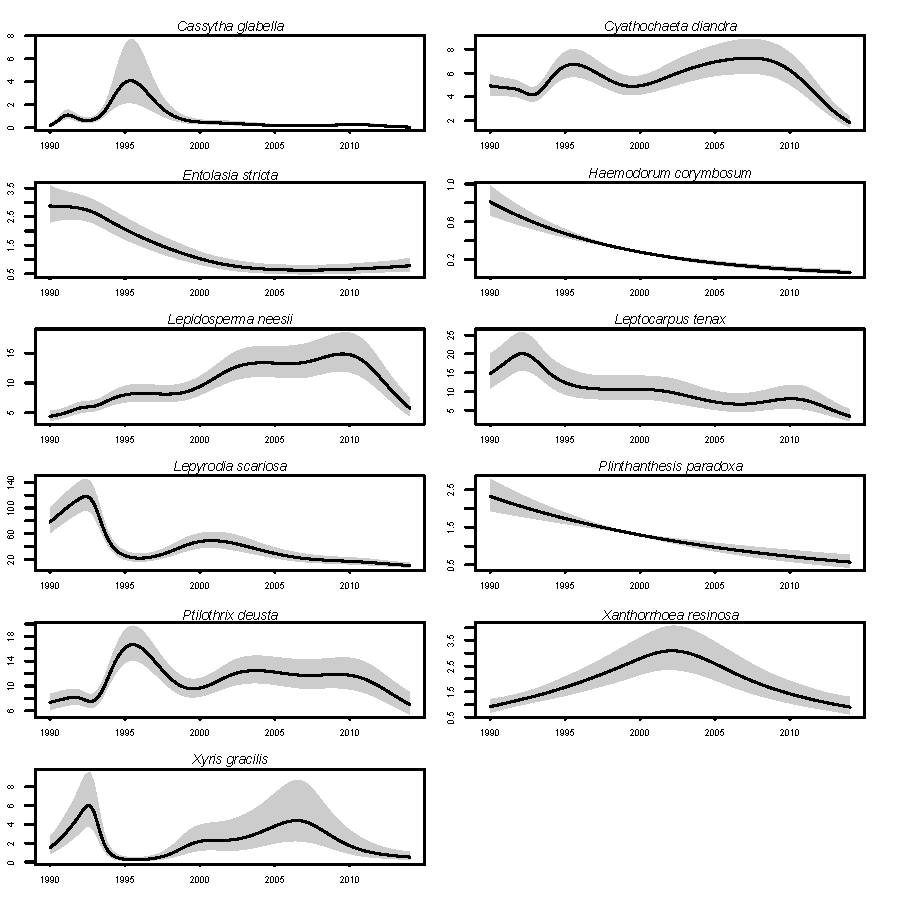
\includegraphics[width=1.0\linewidth]{timeplots}\\   
\end{figure}


\begin{table}[H]
  \centering
  \flushleft\textbf{Table S5.1.} Negative and positive pairwise environmental and residual correlations in each of the four plot clusters. 
    \begin{tabular}{lllll}
    \toprule
          & \multicolumn{2}{l}{No. sig. env. correlations} & \multicolumn{2}{l}{No. sig. res. correlations} \\
    \midrule
          & -ve   & +ve   & -ve   & +ve \\
    deep soil-moisture & 6,0,1,0 & 12,2,4,13 & 8,11,7,0 & 10,14,30,41 \\
    shallow soil-moisture & 2,0,4,0 & 3,3,2,0 & 10,10,5,0 & 17,9,16,42 \\
    pH    & 0,0,3,0 & 1,1,11,0 & 7,10,6,0 & 11,13,23,41 \\
    total iron & 2,0,2,0 & 2,1,3,1 & 10,11,7,0 & 6,8,17,41 \\
    phosphorous & 4,0,9,3 & 3,5,7,3 & 12,11,4,0 & 7,10,26,34 \\
    organic carbon & 1,0,6,0 & 0,0,10,16 & 8,10,6,0 & 6,12,27,39 \\
    exchangeable aluminium & 2,0,2,6 & 4,8,2,12 & 10,16,5,0 & 15,20,25,41 \\
    exchangeable magnesium & 3,0,5,1 & 3,1,9,8 & 10,11,6,0 & 11,13,28,41 \\
    cation exchange capacity & 1,0,5,1 & 2,3,6,0 & 8,13,5,0 & 14,10,21,43 \\
    \bottomrule
    \end{tabular}%
  \label{tab:addlabel}%
\end{table}%

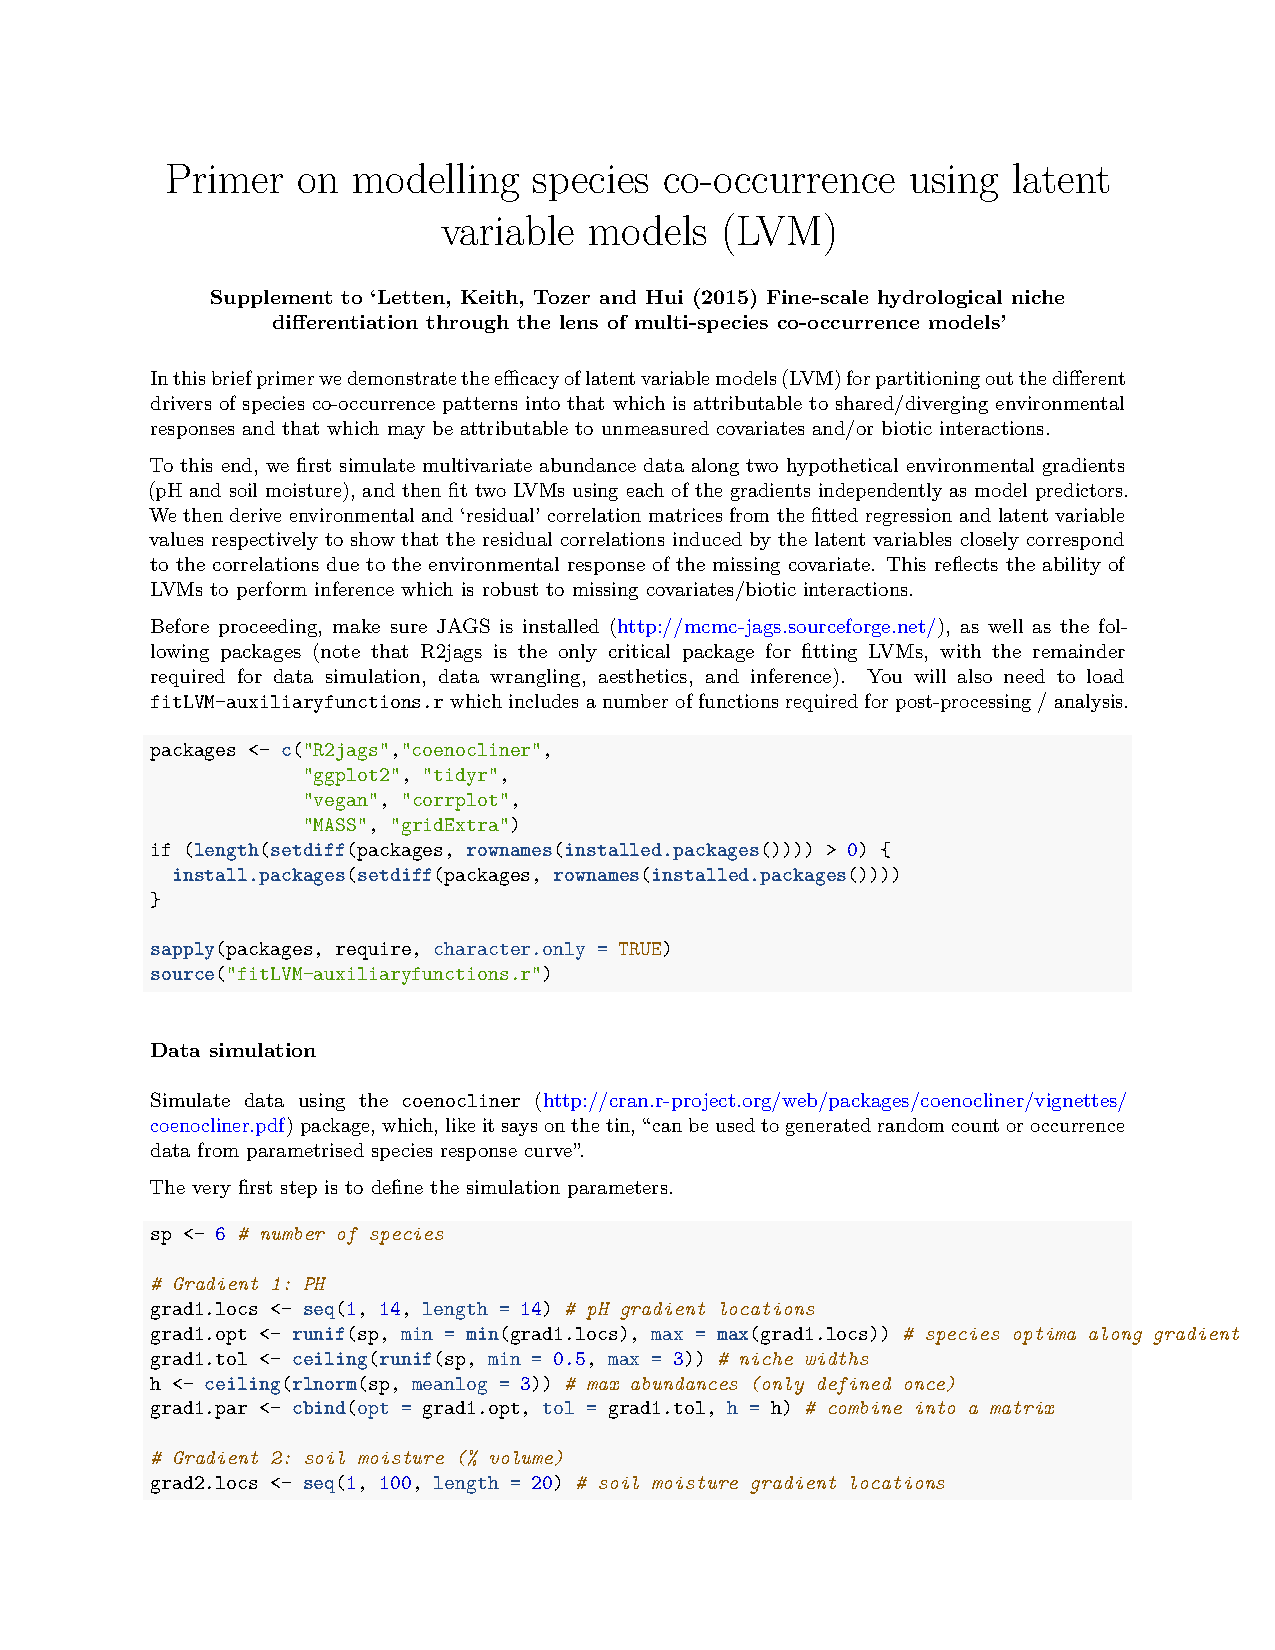
\includepdf[pages={-}, offset=0.4cm 0cm,  addtotoc= {1,section,1,LVM Primer,hlabel}]{Appendix4/LVM-primer.pdf}

\subsection{fitLVM-auxiliaryfunctions.R}

\begin{verbatim}
##########################################
## Auxilary functions for fitting LVMs  ##
##########################################

## Calculate the correlation between spp due to shared/diverging env responses
extract.env.cor <- function(fit.mod, X, y) {		
	n.species <- ncol(y)
	fit.mcmcBase <- fit.mod$BUGSoutput
	mcmc.runs <- mcmc(fit.mcmcBase$sims.matrix, start = 1, 
                    thin = fit.mcmcBase$n.thin) 
	rm(fit.mcmcBase)
		
	all.shared.env.mat <- matrix(0,nrow(mcmc.runs),n.species^2)

	## For each MCMC sample, find the correlation between spp responses
	for(t in 1:nrow(mcmc.runs)) { 
		cw.spp.coef <- matrix(mcmc.runs[t,grep("spp.coef\\[",colnames(mcmc.runs))],
                          n.species,byrow=F)
		eta.mat <- X%*%t(cw.spp.coef) ## On linear predictor scale
		all.shared.env.mat[t,] <- as.vector(cor(eta.mat))
		}

	## Average/Median over the MCMC samples
	env.mat.mean <- sig.env.mat.mean <- matrix(apply(all.shared.env.mat,2,mean),
                                             n.species,byrow=F)
	env.mat.median <- sig.env.mat.median <- matrix(apply(all.shared.env.mat,2,median),
                                                 n.species,byrow=F)
		
	get.cor.intervals <- HPDinterval(as.mcmc(all.shared.env.mat), prob = 0.95)	
	id.sign.cors <- which(get.cor.intervals[,1] > 0 | get.cor.intervals[,2] < 0)	
	sig.env.mat.mean[-id.sign.cors] <- 0
	sig.env.mat.median[-id.sign.cors] <- 0
	
	return(list(envcor.mean = env.mat.mean, 
              envcor.median = env.mat.median, 
              sig.envcor.mean = sig.env.mat.mean, 
              sig.envcor.median = sig.env.mat.median))
	}
	
## Produce the residual correlation
extract.residual.cor <- function(fit.mod, X, y) {
	fit.mcmcBase <- fit.mod$BUGSoutput
	mcmc.runs <- mcmc(fit.mcmcBase$sims.matrix, 
                    start = 1, 
                    thin = fit.mcmcBase$n.thin)
	rm(fit.mcmcBase)

	n.species <- ncol(y)
	n.sites <- nrow(y)
	Tau.arr <- matrix(NA,nrow(mcmc.runs),n.species^2)
	for(t in 1:nrow(mcmc.runs)) { 
		lvs <- matrix(mcmc.runs[t,grep("LV",colnames(mcmc.runs))],
                  n.sites,byrow=F)
		lv.coefs <- matrix(mcmc.runs[t,grep("lv.coef",colnames(mcmc.runs))],
                       n.species,byrow=F)
		Tau.arr[t,] <- as.vector(cor(lvs%*%t(lv.coefs))) }
		
	## Average/Median over the MCMC samples
	Tau.mat.mean <- sig.Tau.mat.mean <- matrix(apply(Tau.arr,2,mean),
                                             n.species,byrow=F)
	Tau.mat.median <- sig.Tau.mat.median <- matrix(apply(Tau.arr,2,median),
                                                 n.species,byrow=F)
		
	get.cor.intervals <- HPDinterval(as.mcmc(Tau.arr), prob = 0.95)	
	id.sign.cors <- which(get.cor.intervals[,1] > 0 | get.cor.intervals[,2] < 0)	
	sig.Tau.mat.mean[-id.sign.cors] <- 0
	sig.Tau.mat.median[-id.sign.cors] <- 0
		
	return(list(rescor.mean = Tau.mat.mean, 
              rescor.median = Tau.mat.median, 
              sig.rescor.mean = sig.Tau.mat.mean, 
              sig.rescor.median = sig.Tau.mat.median))
	}
	
## Produce mean and median point estimates from fit
extract.params <- function(fit.mod) {
	fit.mcmcBase <- fit.mod$BUGSoutput
	mcmc.runs <- mcmc(fit.mcmcBase$sims.matrix, start = 1, 
                    thin = fit.mcmcBase$n.thin) 
	rm(fit.mcmcBase)
	n.species <-  length(grep("spp.int",colnames(mcmc.runs)))

	all.spp.coef <- mcmc.runs[,grep("spp.coef",colnames(mcmc.runs))]
	spp.coef.mean <- matrix(apply(all.spp.coef,2,mean),n.species,byrow=F)	
	spp.coef.median <- matrix(apply(all.spp.coef,2,median),n.species,byrow=F)	
	
	all.spp.int <- mcmc.runs[,grep("spp.int",colnames(mcmc.runs))]
	spp.int.mean <- apply(all.spp.int,2,mean)
  spp.int.median <- apply(all.spp.int,2,median)	
	
	all.spp.phi <- mcmc.runs[,grep("spp.phi",colnames(mcmc.runs))]
	spp.phi.mean <- apply(all.spp.phi,2,mean)
  spp.phi.median <- apply(all.spp.phi,2,median)	

	all.mu.beta <- mcmc.runs[,grep("mu.beta",colnames(mcmc.runs))]
	mu.beta.mean <- apply(all.mu.beta,2,mean)
  mu.beta.median <- apply(all.mu.beta,2,median)	

	all.tau.beta <- mcmc.runs[,grep("tau.beta",colnames(mcmc.runs))]
	tau.beta.mean <- apply(all.tau.beta,2,mean)
  tau.beta.median <- apply(all.tau.beta,2,median)	

	return(list(spp.coef.mean = spp.coef.mean, spp.coef.median = spp.coef.median, 
              spp.int.mean = spp.int.mean, spp.int.median = spp.int.median, 
              spp.phi.mean = spp.phi.mean, spp.phi.median = spp.phi.median, 
              mu.beta.mean = mu.beta.mean, mu.beta.median = mu.beta.median, 
              tau.beta.mean = tau.beta.mean, tau.beta.median = tau.beta.median))
	}
\end{verbatim}